\documentclass{standalone}
\usepackage{tikz}
\usepackage{ctex,siunitx,bm}
\setCJKmainfont{Noto Serif CJK SC}
\usepackage{tkz-euclide,ninecolors}
\usepackage{amsmath}
\usetikzlibrary{patterns, calc}
\usetikzlibrary {decorations.pathmorphing, decorations.pathreplacing, decorations.shapes,}
\begin{document}
\small
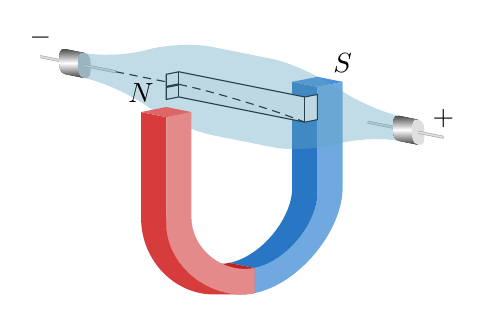
\begin{tikzpicture}[>=latex,scale=0.8]
  \useasboundingbox(-3.4,1.1)rectangle(3.4,-3.3);
  \fill[azure7](0.2,-3.114)..controls(0.9,-2.974)and(1.6,-2.134)..(1.6,-1.434)--(1.6, 0.240)--(1.2, 0.160)--(1.2,-1.514)..controls(1.2,-2.014)and(0.7,-2.614)..(0.2,-2.714)--cycle;
  \fill[azure5]( 0.2,-2.714)..controls( 0.7,-2.614)and( 1.2,-2.014)..( 1.2,-1.514)--( 1.2, 0.160)--( 0.8, 0.240)--( 0.8,-1.434)..controls( 0.8,-1.934)and( 0.3,-2.534)..(-0.2,-2.634)--cycle;
  \fill[azure6](0.8,0.24)--(1.2,0.32)--(1.6,0.24)node[above,text=black]{$S$}--(1.2,0.16)--cycle;
  \foreach \x in {80,60,40,20}
  {
    \draw[line width={sin(\x)},gray!\x](-3.2,0.64)--(-2.5,0.5);
    \draw[line width={sin(\x)},gray!\x](2,-0.4)--(2.7,-0.54);
  }
  \fill[top color=darkgray,bottom color=darkgray,middle color=white]
  (-2.8,0.36)..controls(-2.9,0.38)and(-2.9,0.48)..(-2.9,0.58)..controls(-2.9,0.68)and(-2.9,0.78)..(-2.8,0.76)--(-2.5,0.70)..controls(-2.6,0.72)and(-2.6,0.62)..(-2.6,0.52)..controls(-2.6,0.42)and(-2.6,0.32)..(-2.5,0.30)--cycle;
  \fill[lightgray](-2.5,0.70)..controls(-2.4,0.68)and(-2.4,0.58)..
  (-2.4,0.48)..controls(-2.4,0.38)and(-2.4,0.28)..
  (-2.5,0.30)..controls(-2.6,0.32)and(-2.6,0.42)..
  (-2.6,0.52)..controls(-2.6,0.62)and(-2.6,0.72)..cycle;
  \foreach \x in {80,60,40,20}
  {
    \draw[line width={sin(\x)},gray!\x](-2,0.4)--(-2.5,0.5);
  }
  \draw[densely dashed](-2,0.4)--(-1,0.2);
  % \draw(-1.5,0.3)--++(120:0.8)node[above]{电子束};
  % \draw(0,0.2)--++(60:0.8)node[above]{荧光屏};
  \draw[fill=lightgray!10](-1.2, 0.36)--(-1.0, 0.40)--( 1.0, 0.00)--( 1.2, 0.04)--( 1.2,-0.36)--( 1.0,-0.40)--(-1.0, 0.00)--(-1.2,-0.04)--cycle;
  \draw[thin](-1,0.4)--(-1,0)(1,0)--(1,-0.4);
  \draw[thick](-1,0.2)--(-1.2,0.16);
  \draw[densely dashed](-1,0.2)..controls(-0.5,0.1)and(0.5,-0.2)..(1,-0.4);
  \fill[cyan!50!gray,opacity=0.4]( 2.50,-0.700)..controls( 2.20,-0.640)and( 1.75,-0.675)..( 1.50,-0.750)..controls( 1.25,-0.825)and( 0.75,-0.850)..( 0.50,-0.800)--(-0.50,-0.600)..controls(-0.75,-0.550)and(-1.25,-0.325)..(-1.50,-0.150)..controls(-1.75, 0.025)and(-2.20, 0.240)..(-2.5,0.30)..controls(-2.6,0.32)and(-2.6,0.42)..  (-2.6,0.52)..controls(-2.6,0.62)and(-2.6,0.72)..(-2.5,0.70)..controls(-2.20, 0.640)and(-1.75, 0.675)..(-1.50, 0.750)..controls(-1.25, 0.825)and(-0.75, 0.850)..(-0.50, 0.800)--( 0.50, 0.600)..controls( 0.75, 0.550)and( 1.25, 0.325)..( 1.50, 0.150)..controls( 1.75,-0.025)and( 2.20,-0.240)..( 2.50,-0.300)--cycle;
  \fill[top color=darkgray,bottom color=darkgray,middle color=white](2.8,-0.36)..controls(2.7,-0.34)and(2.7,-0.44)..(2.7,-0.54)..controls(2.7,-0.64)and(2.7,-0.74)..(2.8,-0.76)--(2.5,-0.70)..controls(2.4,-0.68)and(2.4,-0.58)..(2.4,-0.48)..controls(2.4,-0.38)and(2.4,-0.28)..(2.5,-0.30)--cycle;
  \fill[lightgray!50](2.7,-0.54)..controls(2.7,-0.44)and(2.7,-0.34)..(2.8,-0.36)..controls(2.9,-0.38)and(2.9,-0.48)..(2.9,-0.58)..controls(2.9,-0.68)and(2.9,-0.78)..(2.8,-0.76)..controls(2.7,-0.74)and(2.7,-0.64)..cycle;
  \foreach \x in {80,60,40,20}
  {
    \draw[line width={sin(\x)},gray!\x](2.8,-0.56)--(3.2,-0.64);
  }
  \node at (3.2,-0.64)[above]{$+$};
  \node at (-3.2,0.64)[above]{$-$};

  \fill[red4](-1.200,-1.994)..controls(-1.200,-2.631)and(-0.620,-3.135)..
  ( 0.011,-3.135)..controls( 0.074,-3.135)and( 0.137,-3.127)..( 0.200,-3.114)--( 0.200,-2.714)--
  (-0.200,-2.634)..controls(-0.700,-2.734)and(-1.200,-2.334)..(-1.200,-1.834)--cycle;
  \fill[red5]( 0.011,-3.135)..controls(-0.620,-3.135)and(-1.200,-2.631)..(-1.200,-1.994)--(-1.200,-0.320)--(-1.600,-0.240)--(-1.600,-1.914)..controls(-1.600,-2.611)and(-1.056,-3.135)..(-0.448,-3.135)--cycle;
  \fill[red7]( 0.200,-2.714)..controls(-0.300,-2.814)and(-0.800,-2.414)..(-0.800,-1.914)--(-0.800,-0.240)--(-1.200,-0.320)--(-1.200,-1.994)..controls(-1.200,-2.631)and(-0.620,-3.135)..( 0.011,-3.135)..controls( 0.074,-3.135)and( 0.137,-3.127)..( 0.200,-3.114)--cycle;
  \fill[red6](-1.2,-0.32)--(-1.6,-0.24)node[text=black,above]{$N$}--(-1.2,-0.16)--(-0.8,-0.24)--cycle;
\end{tikzpicture}
\end{document}